%%%%%%%%%%%%%%%%%%%%%%%%%%%%%%%%%%%%%%%%%
% Plasmati Graduate CV
% LaTeX Template
% Version 1.0 (24/3/13)
%
% This template has been downloaded from:
% http://www.LaTeXTemplates.com
%
% Original author:
% Alessandro Plasmati (alessandro.plasmati@gmail.com)
%
% License:
% CC BY-NC-SA 3.0 (http://creativecommons.org/licenses/by-nc-sa/3.0/)
%
% Important note:
% This template needs to be compiled with XeLaTeX.
% The main document font is called Fontin and can be downloaded for free
% from here: http://www.exljbris.com/fontin.html
%
%%%%%%%%%%%%%%%%%%%%%%%%%%%%%%%%%%%%%%%%%

\documentclass[a4paper,13pt]{article}
\usepackage[margin=0in]{geometry}
\usepackage{layout}
\usepackage{a4wide}
\usepackage{fontspec}
\addtolength{\voffset}{-0.9in}
\addtolength{\footskip}{1mm}
\usepackage{hyperref}
\usepackage{setspace}
\defaultfontfeatures{Mapping=tex-text}
\usepackage{xunicode,xltxtra,url,parskip} % Formatting packages
\usepackage[usenames,dvipsnames]{xcolor} % Required for specifying 
\usepackage[big]{layaureo} % Margin formatting of the A4 page, an 
\usepackage{hyperref} % Required for adding links	and customizing them
\definecolor{linkcolour}{rgb}{0,0.2,0.6} % Link color
\hypersetup{colorlinks,breaklinks,urlcolor=linkcolour,linkcolor=linkcolour} % Set link colors throughout the document

\usepackage{titlesec} % Used to customize the \section command
\titleformat{\section}{ \bfseries\raggedright}{}{0cm}{}[] % Text formatting of sections

\titlespacing{\section}{0pt}{0pt}{-10pt} % Spacing around sections
\usepackage{changepage}
\usepackage{fontawesome}
{\renewcommand{\arraystretch}{0.83} % Adjusts the spaces between table columns


\begin{document}

\pagestyle{empty} % Removes page numbering

\font\fb=''[cmr9]'' % Change the font of the \LaTeX command under the skills section

%----------------------------------------------------------------------------------------
%	NAME AND CONTACT INFORMATION
%----------------------------------------------------------------------------------------

\par{\hspace{5cm}\huge Aly \textsc{Saleh}\par} % Your name


% \raggedright{Personal Data}

\begin{adjustwidth}{-3cm}{}

\begin{tabular}{rl}
	&	\textbf{Phone}: 017672763029, 
		  \textbf{E-mail}: 	\href{mailto:aly.mostafa15@gmail.com}{aly.mostafa15@gmail.com},
 		  \textbf{Nationality}: Egyptian,  \faLinkedin: \href{https://de.linkedin.com/in/aly-saleh-ba948164}{Aly Saleh}
 
	\\&	\textbf{Address}: Riesengebirgstraße, 80993, Munich, 
		 \textbf{Date of Birth}: 1 December 1991,		 \faGithub:  \href{https://github.com/SalehAly}{@SalehAly}\\

\end{tabular}
\begin{figure}
	\begin{center}
	\hspace{14cm} \vspace{-3cm} 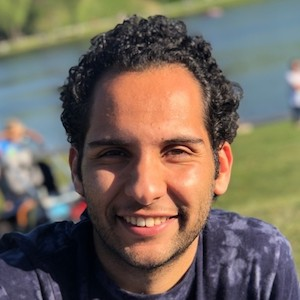
\includegraphics[scale=0.07]{me.jpg}	
	\end{center}

\end{figure}



%\end{adjustwidth}


%----------------------------------------------------------------------------------------
%	WORK EXPERIENCE 
%----------------------------------------------------------------------------------------

\section{Work Experience}
\rule[0pt]{20cm}{0.5pt}

\begin{tabular}{r|p{17.5cm}}
		
		\textsc{Present} & \textbf{Junior Software Developer} at \textbf{ CHECK24 Vergleichsportal GmbH}, Munich \\
		\textsc{Jul 2017} & \footnotesize{
			- Using Springboot, Docker, Redis, ActiveMQ and Kubernetes to build Microservices for online loan products at Kredite24.
		}
		\\ \multicolumn{2}{c}{}\\
		
\textsc{May 2017} & \textbf{Work Student Back-end Software Engineer} at \textbf{IDgard.de}, Munich \\
\textsc{Oct 2015} & \footnotesize{
	- Implemented a proof of concept \textbf{JAX-RS} back end that is at least \textbf{twice} as fast than the current one.\newline
	- Ran several performance and stress tests using \textbf{Apache JMeter} \newline
	- Researched on how to write a new API specification that is RESTful using current trends in technology \textbf{swagger.io}. \newline
	- Participated in a research in order to transfer our back-end into \textbf{Micro-services} with \textbf{Message queues.}
}
\\ \multicolumn{2}{c}{}\\

%------------------------------------------------

\textsc{Oct 2015} & \textbf{Work Student Java Developer} at \textbf{HRForecast.de}, Munich \\
\textsc{May 2015} & \footnotesize{ - Enhanced an analytics tool mainly written in Java with Vaadin framework. \newline
- Refracted the code base since it lacked extensibility and scalability.
} \\ 
\multicolumn{2}{c}{} \\

%------------------------------------------------

\textsc{Mar 2015} & \textbf{Back-end Software Engineer} at \href{http://desktop.bey2ollak.com/features-mentions/}{\textbf{Bey2ollak}}, Cairo \\
\textsc{Sep 2012} & 

\footnotesize{
	- Had hands on multiple web and database servers, maintained back-end requests adding more features and solving problems (bugs).\newline 
	- Transferred \textbf{MySQL} database into SAN storage, used JMeter for functional and load testing, benchmarked MySQL using sysbench.\newline
	- Developed many \textbf{JSP} tools and wrote \textbf{bash} scripts to dump the database and synchronize the logs to other servers.\newline
	- Participated in a research for handling big data using the \textbf{ELK} stack.
}
\end{tabular}

%------------------------------------------------


%----------------------------------------------------------------------------------------
%	EDUCATION
%----------------------------------------------------------------------------------------


\section{Education}
\rule[0pt]{20cm}{0.5pt}

\begin{tabular}{r|p{17.5cm}}
		
%------------------------------------------------

\textsc{Present} & \textbf{M.Sc. Informatik Student}, 4rth Semester\\ \textsc{April} 2015 & \normalsize\textbf{Technische Universität München (TUM)}, Germany\footnotesize \hfill| \normalsize \textsc{Gpa}: 2.0\\
& \small\emph{Major: Software Engineering, Minor: Distributed Systems}
\\ \multicolumn{2}{c}{} \\

\textsc{Present}&
\textbf{M.Sc Thesis Context-Sensitive Pervasive Computing for Smart Cities}\\
%& \href{https://github.com/SalehAly/master-thesis}{Topic repository} - Keywords: \href{https://www.google.de/search?q=Pervasive+Computing}{\#Pervasive Computing}, \href{https://www.google.de/search?q=context+sensitive}{\#Context Sensitive}, \href{nodered.org}{\#IBM Node-red} \\
& Expected Graduation date \textbf{June 2017} 
\\ \multicolumn{2}{c}{} \\


\textsc{July} 2013 & \textbf{Bachelor Degree in Computer Science and Engineering},\\ \textsc{July} 2008& \normalsize\textbf{The German University in Cairo}, Cairo\\
& \small{Faculty of Media Engineering and Technology} \small{Department of Computer Science and Engineering}  \footnotesize \hfill| \normalsize \textsc{Gpa}: 1.86
\\\multicolumn{2}{c}{} \\

\textsc{May} 2012 & \textbf{Bachelor Project, The University of Ulm}, Germany\\
\textsc{Mar} 2012 & \small{Faculty of Computer Science, Department of Software Engineering and} \small{Compiler Construction.} 
% \footnotesize{Thesis: ``CHR-based Text Mining and Classification of Google Search Results''}   \footnotesize{Advisor: Prof. Thom \textsc{Fr{\"u}hwirth}} \hfill| \footnotesize \normalsize
 \hfill| \footnotesize \normalsize \textsc{Gpa}: A-/A 
\\
\end{tabular}


%----------------------------------------------------------------------------------------
%	SCHOLARSHIPS AND ADDITIONAL INFO
%----------------------------------------------------------------------------------------



\section{Highlights} \label{praktikum}
\rule[0pt]{20cm}{0.5pt}

\begin{tabular}{r|p{17.5cm}}
	\textsc{Projects} &Algorithms For Programming Contests: Learned new efficient algorithms widely used in programming contests. 
	\\\multicolumn{1}{c}{} \\
	&IOS Praktikum: Participated in \href{https://www1.in.tum.de/lehrstuhl_1/component/content/article/733#CHEST}{CHEST}; A Cyber-Physical System that provides live health data to action forces in critical situations. Learned \textbf{Swift 2.0} and Implemented a back end system using \textbf{Node.js}, \textbf{MQTT} and \textbf{MongoDB}. \\\multicolumn{1}{c}{} \\
	
	&Software Engineering for Business Applications: Used \textbf{Play} framework in order to implement a business case
	after creating a \textbf{Business Model Canvas} and \textbf{Value Proposition Canvas}.
	\\\multicolumn{1}{c}{} \\
	\textsc{Seminars} &Internet-Scale Distributed Systems Seminar: Gave a presentation and wrote a report about \textbf{redis} replication, clustering and persistence. \\
\end{tabular}


%----------------------------------------------------------------------------------------
%	COMPUTER SKILLS 
%----------------------------------------------------------------------------------------

\section{Programming Knowledge}
\rule[0pt]{20cm}{0.5pt}

\begin{tabular}{r|p{17.5cm}}

\textbf{Excellent}  & Java, Servlets, JAX-RS, JSP's, JPA,  MySQL, Linux, GIT, Maven, JIRA, Confluence, Bamboo.
\\\multicolumn{2}{c}{} \\
\textbf{Good}  &  Spring boot, Google Guice, Swagger, Docker, Load Testing "Jmeter", Logstash, Kibana (ELK Stack), Play
 
  Javascript, Nodejs, MongoDB, Vaadin, Jquery, JqueryUI, Bash Scripts {\fb \LaTeX}
\\\multicolumn{2}{c}{} \\
\textbf{Fair}  & Python, Swift, Android, ElasticSearch
\\
\end{tabular}



%----------------------------------------------------------------------------------------
%	LANGUAGES
%----------------------------------------------------------------------------------------

\section{Languages and Courses}
\rule[0pt]{20cm}{0.5pt}

	\begin{tabular}{rp{17.5cm}}
\textbf{English}: Fluent, 
\textbf{German}: Good Knowledge \textbf{B1}, 
\textbf{Arabic}: Mother Tongue\\
\end{tabular}



\section{Tech. Interests}
\rule[0pt]{20cm}{0.5pt}        \\
Microservices, Reactive Manifesto, GO lang,  Internet Of Things, New programming languages, Scalability, Security.
\end{adjustwidth}

%----------------------------------------------------------------------------------------
%	INTERESTS AND ACTIVITIES
%----------------------------------------------------------------------------------------

%\section{Masters Courses} \label{courses}

%\begin{adjustwidth}{-2cm}{}
%Advanced Topics on Software Testing, 
%Parallel Programming, 
%Project Organization and Management for Software Engineering, 
%Security Engineering, 
%Seminar on Internet-scale Distributed Systems, 
%Software Engineering For Business Applications, 
%Software Design Patterns, 
%User Modeling and Recommender Systems, 
%Value Based Management.
%\end{adjustwidth}

%\section{Interests and Activities}
%\begin{adjustwidth}{-2cm}{}
%Internet Of Things, New programming languages, Scalability, Privacy, Meetups, %\\Hackathons and new Technologies 
%Traveling and Exploration, Charity, Fishing, Football, Volleyball and Gymnastics.
%\end{adjustwidth}



%----------------------------------------------------------------------------------------

%\newpage

%----------------------------------------------------------------------------------------
%	GRADE TABLES
%----------------------------------------------------------------------------------------

%\par{\centering\Large \hypertarget{grds}{Master of Science in \textsc{Finance}}\par}\large{\centering Grades\par}\normalsize

%\begin{center}
%\begin{tabular}{lcc}
%\multicolumn{1}{c}{\textsc{Exam}} & \textsc{Grade}&\textsc{Credit Hrs}\\ \hline
%Corporate Finance (Valuation) & 25 & 6\\
%Financial Statement Analysis & 28 & 6\\
%Statistics & 27 & 6\\
%Theory of Finance & 26 & 6\\
%Quantitative Methods for Finance & 30 & 6\\
%Econometrics & 24 & 6\\
%Derivatives & 31 & 6\\
%Management of Financial and Insurance Companies & 30 & 6\\
%Business Law & 31 & 6\\
%Investment Banking	& 28 & 6\\ \\		
%Behavioral Models for Economics and Finance	 & 29 & 6\\
%Numerical Methods for Finance & 29 & 6\\
%Advanced Derivatives & 30 & 6\\
%Fixed Income (Advanced Methods) & 30 & 6\\ \\
%English Language & 30 &	4\\
%French Language & 31 &	4\\	
%Internship & & 8\\		
%Final Thesis & & 20\\	
%& Total & 120\\\cline{2-3}
%&\textsc{Gpa}&\textbf{8.0}
%\end{tabular}
%\end{center}
%\bigskip
%\hrule
%\bigskip

%------------------------------------------------

%\bigskip

%\par{\centering\Large \hypertarget{grds_usc}{Exchange Program at \textsc{usc}, Los Angeles}\par}\large{\centering %Grades\par}\normalsize

%\begin{center}
%\begin{tabular}{lcc}
%\multicolumn{1}{c}{\textsc{Exam}} & \textsc{Grade} & \textsc{Grade Points}\\ 
%\hline
%Corporate Financial Strategy & A & 4\\
%Derivatives & A & 4\\
%Money, Credit, and Banking & A & 4\\
%Business Strategy & A- & 3.5\\
%& &\\\cline{2-3}
%& \textsc{Gpa} & \textbf{3.875}
%\end{tabular}
%\end{center}

%----------------------------------------------------------------------------------------

\end{document}
